
%\section{qPCR Copy Number Calling}

\begin{figure}[h]
%\begin{center}
    \centering
    \begin{subfigure}[c]{.5\textwidth}
        %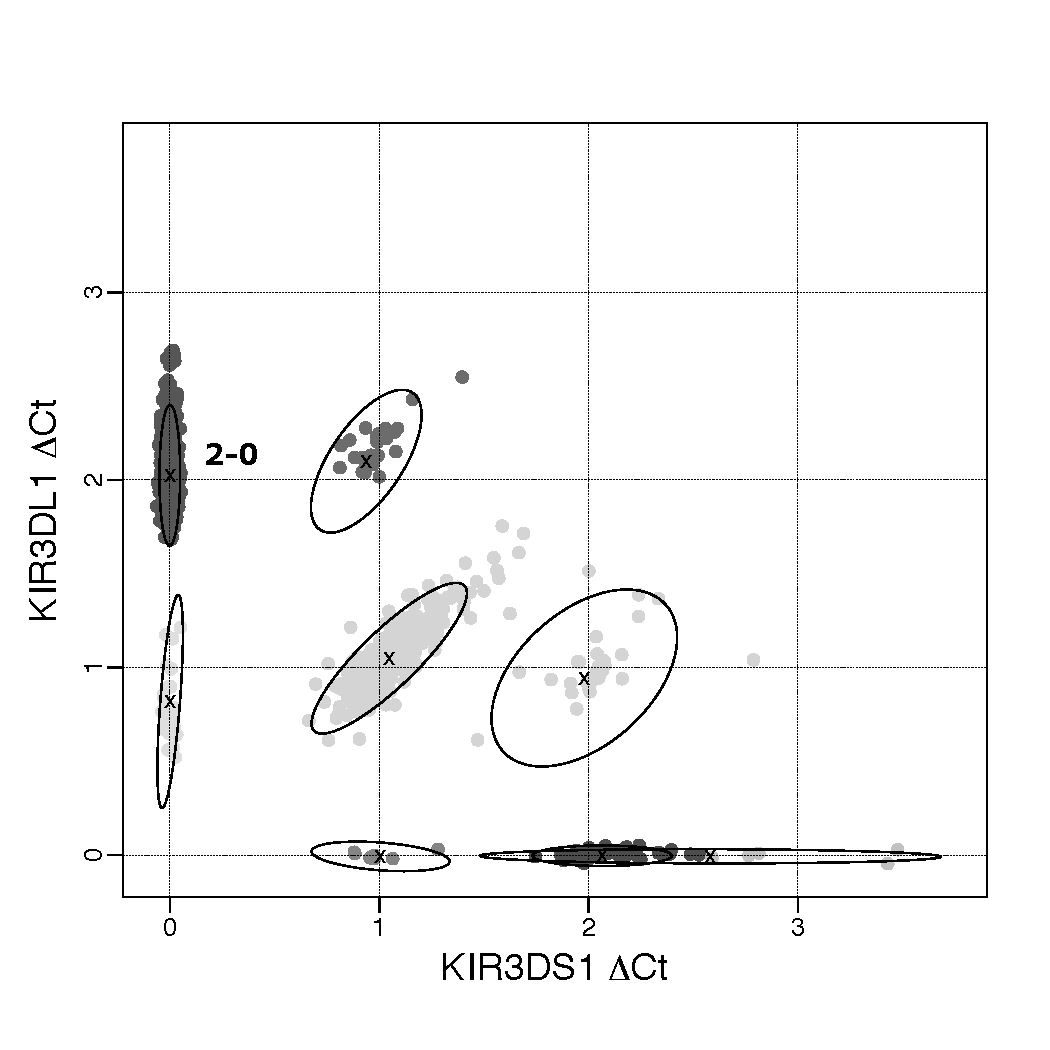
\includegraphics[scale=.5] {figures/genotyping-graytone.pdf}
        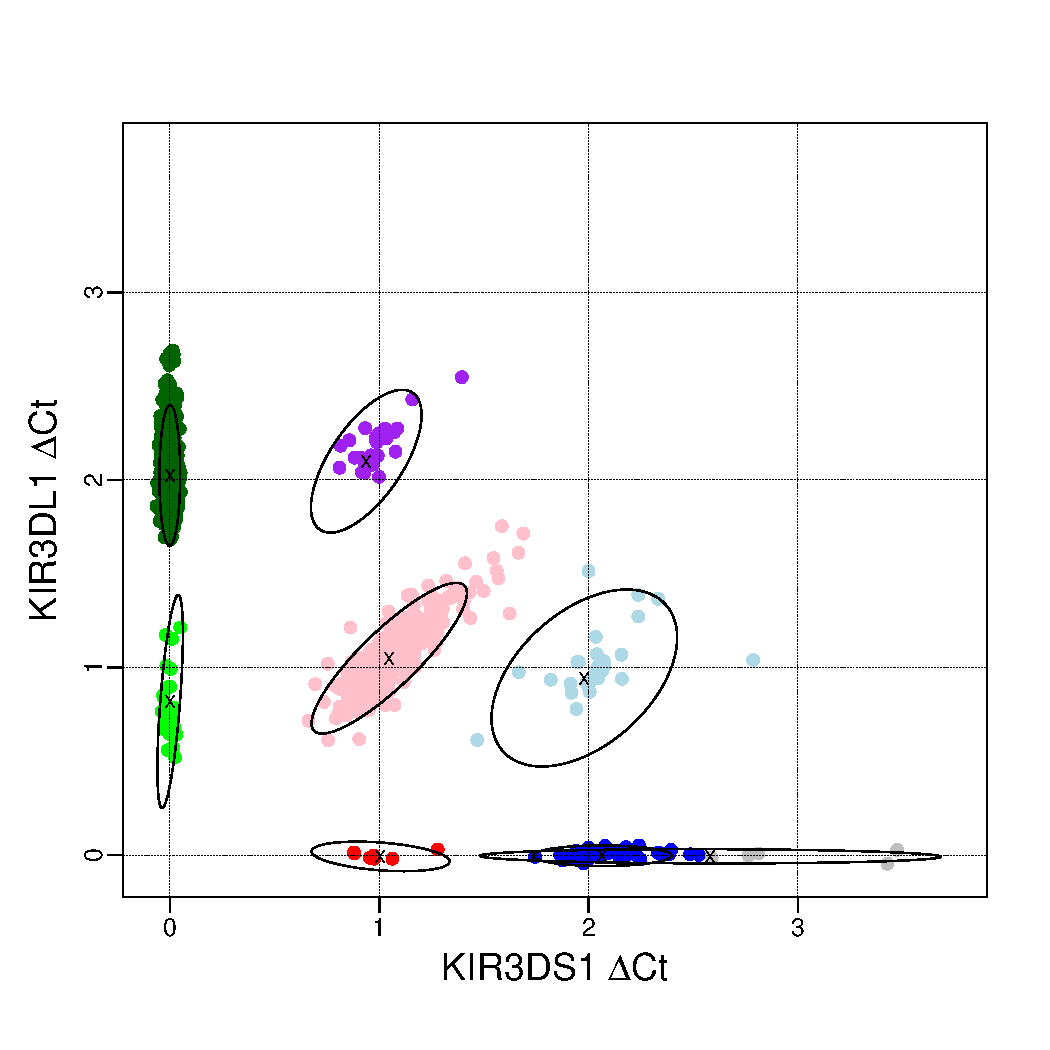
\includegraphics[scale=.5] {figures/genotyping.pdf}
    \end{subfigure}
    \begin{subfigure}[c]{.4\textwidth}\footnotesize
        %\texttt{
    \begin{tabular}{crrr}
      \toprule
      {\tiny KIR3DS1-KIR3DL1} & \multicolumn{3}{c}{count (percentage)} \\
          Copy Number & cases & controls & total \\ 
      \hline
        0-2 & 444 (59.44) & 446 (61.35) & 890 (60.38) \\ 
        1-1 & 229 (30.66) & 207 (28.47) & 436 (29.58) \\ 
        2-0 & 26 (3.48) & 28 (3.85) & 54 (3.66) \\ 
        2-1 & 15 (2.01) & 16 (2.2) & 31 (2.1) \\ 
        1-2 & 13 (1.74) & 14 (1.93) & 27 (1.83) \\ 
        0-1 & 13 (1.74) & 11 (1.51) & 24 (1.63) \\ 
        1-0 & 4 (0.54) & 3 (0.41) & 7 (0.47) \\ 
        3-0 & 3 (0.4) & 2 (0.28) & 5 (0.34) \\ 
      \midrule
      .-2 & 457 (61.18) & 460 (63.27) & 917 (62.21) \\ 
      .-1 & 257 (34.4) & 234 (32.19) & 491 (33.31) \\ 
      .-0 & 33 (4.42) & 33 (4.54) & 66 (4.48) \\ 
      \midrule
        0-. & 457 (61.18) & 457 (62.86) & 914 (62.01) \\ 
        1-. & 246 (32.93) & 224 (30.81) & 470 (31.89) \\ 
        2-. & 41 (5.49) & 44 (6.05) & 85 (5.77) \\ 
        3-. & 3 (0.4) & 2 (0.28) & 5 (0.34) \\ 
      \midrule
      Total &  747 (100) & 727 (100) & 1474 (100)\\ 
      \bottomrule
    \end{tabular}
    %}
    \end{subfigure}
    \caption{
        \label{figure:fuzzy-genotyping}
        On the left,
        the median normalised $\Delta$ct values for KIR3DS1 and KIR3DL1 are shown with
        the results of clustering into the eight genotype groups indicated by colouring points according to the group
        %the mixture of bivariate Gaussian clustering of the eight genotype groups.
        with the greatest posterior probability.
        The three most common genotype groups are the ones with normal copy numbers:
        KIR3DL1 homozygous (dark green), KIR3DL1/S1 heterozygous (pink) and KIR3DS1 homozygous (dark blue).
        %The rarer ones are: 2/1 (light blue), 1/2 (purple), 0/1 (light green), 1/0 (red) and 3/0 (gray).
        The ellipses delimit the $95^{th}$ percentile.
        On the right, the counts of the most probable bivariate genotypes are shown for cases and controls.
    }
\end{figure}



%\section{HLA typing}



\clearpage

%\section{T1D Association}


%\subsection{SNP}

\begin{table}[h]\footnotesize
%\begin{center}
    %\texttt{ %}
\begin{tabularx}{\textwidth}{ccrrrr|crrrr}
  \multicolumn{1}{l}{\bf{a)}} & \multicolumn{5}{c}{qPCR} & \multicolumn{5}{c}{SNP} \\
  \hline
    KIR3DS1/L1 & case:control & total & OR & 95\%CI & p-value & case:control & total  & OR & 95\%CI & p-value \\
  \hline
    0-2 & 444:446 &  890 & 1.00 &  &  & 4091:3220 &  7311  & 1.00 &  &  \\
    1-1 & 229:207 &  436 & 1.11 & 0.88-1.40 & 0.3673 & 2056:1628 &  3684  & 0.99 & 0.92-1.08 & 0.8828 \\
    2-0 & 26:28 &   54 & 0.92 & 0.52-1.61 & 0.7713 & 231:223 &   454  & 0.82 & 0.67-0.99 & 0.0349 \\
    2-1 & 15:16 &   31 & 0.94 & 0.46-1.93 & 0.8695 & 116:104 &   220  & 0.88 & 0.67-1.15 & 0.3422 \\
    1-2 & 13:14 &   27 & 0.93 & 0.43-2.01 & 0.8587 & 101:73 &   174  & 1.09 & 0.80-1.48 & 0.5833 \\
    0-1 & 13:11 &   24 & 1.19 & 0.53-2.68 & 0.6794 & 116:79 &   195  & 1.16 & 0.87-1.54 & 0.3273 \\
    1-0 & 4:3 &    7 & 1.34 & 0.30-6.02 & 0.7031 & 24:20 &    44  & 0.94 & 0.52-1.71 & 0.8509 \\
    3-0 & 3:2 &    5 & 1.52 & 0.27-8.62 & 0.6369 & 9:15 &    24  & 0.47 & 0.21-1.08 & 0.0756 \\
  \hline
    & 747:727 & 1474 &  &  &  & 6744:5362 & 12,106  &  & &  \\
  \\
  \multicolumn{1}{l}{\bf{b)}} & \multicolumn{5}{c}{qPCR} & \multicolumn{5}{c}{SNP} \\
  \hline
    KIR3DL1 & case:control & total & OR & 95\%CI & p-value & case:control & total  & OR & 95\%CI & p-value \\
  \hline
    .-2 & 457:460 &  917 & 1.00 &  &  & 4192:3293 &  7485  & 1.00 &  &  \\
    .-1 & 257:234 &  491 & 1.11 & 0.89-1.38 & 0.3702 & 2288:1811 &  4099  & 0.99 & 0.92-1.07 & 0.8464 \\
    .-0 & 33:33 &   66 & 1.01 & 0.61-1.66 & 0.9795 & 264:258 &   522  & 0.80 & 0.67-0.96 & 0.0159 \\
  \hline
    & 747:727 & 1474 &  &  &  & 6744:5362 & 12,106  &  & &  \\
  \\
  \multicolumn{1}{l}{\bf{c)}} & \multicolumn{5}{c}{qPCR} & \multicolumn{5}{c}{SNP} \\
  \hline
    KIR3DS1 & case:control & total & OR & 95\%CI & p-value & case:control & total  & OR & 95\%CI & p-value \\
  \hline
    0-. & 457:457 &  914 & 1.00 &  &  & 4207:3299 &  7506  & 1.00 &  &  \\
    1-. & 246:224 &  470 & 1.10 & 0.88-1.37 & 0.4096 & 2181:1721 &  3902  & 0.99 & 0.92-1.07 & 0.8750 \\
    2-. & 41:44 &   85 & 0.94 & 0.60-1.47 & 0.7787 & 347:327 &   674  & 0.83 & 0.71-0.97 & 0.0224 \\
    3-. & 3:2 &    5  & 1.24 & 0.21-7.28 & 0.8084 & 9:15 &    24  & 0.47 & 0.21-1.08 & 0.0741 \\
  \hline
    & 747:727 & 1474 &  &  &  & 6744:5362 & 12,106  &  & &  \\
\end{tabularx}
    \caption{
        \label{table:kir-t1d}
        No evidence of a significant joint or marginal effect of \emph{KIR3DS1/L1} copy number with T1D in qPCR dataset, 747 cases and 727 controls, and in SNP dataset, 6,744 cases and 5,362 controls.
    }
\end{table}


%\subsection{qPCR}


\begin{table}[h]\footnotesize
\begin{tabularx}{\textwidth}{ccrrrr|crrrr}
  \multicolumn{11}{c}{HLA-Bw4-80 subset} \\
  \multicolumn{1}{l}{\bf{a)}} & \multicolumn{5}{c}{qPCR} & \multicolumn{5}{c}{SNP} \\
  \hline
    KIR3DS1/L1 & case:control & total & OR & 95\%CI & p-value & case:control & total  & OR & 95\%CI & p-value \\
  \hline
    0-2 & 259:286 & 545 & 1.00 &  &  & 1025:1156 & 2181  & 1.00 &  &  \\
    1-1 & 123:128 & 251 & 1.06 & 0.79-1.43 & 0.6976 & 556:583 & 1139  & 1.08 & 0.93-1.24 & 0.3194 \\
    2-0 & 16:15 &  31 & 1.22 & 0.58-2.57 & 0.5985 & 61:87 &  148  & 0.79 & 0.56-1.11 & 0.1733 \\
    2-1 & 7:13 &  20 & 0.59 & 0.23-1.51 & 0.2754 & 32:40 &   72  & 0.90 & 0.56-1.45 & 0.6695 \\
    1-2 & 8:8 &  16 & 1.10 & 0.41-2.98 & 0.8450 & 27:32 &   59  & 0.95 & 0.57-1.60 & 0.8513 \\
    0-1 & 10:7 &  17 & 1.58 & 0.59-4.20 & 0.3621 & 36:26 &   62  & 1.56 & 0.94-2.60 & 0.0876 \\
    1-0 & 2:1 &   3 & 2.21 & 0.20-24.50 & 0.5187 & 7:3 &   10  & 2.63 & 0.68-10.19 & 0.1614 \\
    3-0 & 3:0 &   3 &  &  &  & 3:1 &    4  & 3.38 & 0.35-32.51 & 0.2910 \\
  \hline
    & 428:458 & 886 &  &  &  & 1747:1928 & 3,675  &  & &  \\
  \\

  \multicolumn{11}{c}{HLA-Bw4-80 subset} \\
  \multicolumn{1}{l}{\bf{b)}} & \multicolumn{5}{c}{qPCR} & \multicolumn{5}{c}{SNP} \\
  \hline
    KIR3DL1 & case:control & total & OR & 95\%CI & p-value & case:control & total  & OR & 95\%CI & p-value \\
  \hline
    .-2 & 267:294 & 561 & 1.00 &  &  & 1052:1188 & 2240  & 1.00 &  &  \\
    .-1 & 140:148 & 288 & 1.04 & 0.78-1.38 & 0.7787 & 624:649 & 1273  & 1.09 & 0.95-1.25 & 0.2414 \\
    .-0 & 21:16 &  37 & 1.45 & 0.74-2.83 & 0.2822 & 71:91 &  162  & 0.88 & 0.64-1.21 & 0.4399 \\
  \hline
    & 428:458 & 886 &  &  &  & 1747:1928 & 3,675  &  & &  \\
  \\
  \multicolumn{11}{c}{HLA-Bw4-80I subset} \\
  \multicolumn{1}{l}{\bf{c)}} & \multicolumn{5}{c}{qPCR} & \multicolumn{5}{c}{SNP} \\
  \hline
    KIR3DS1 & case:control & total & OR & 95\%CI & p-value & case:control & total  & OR & 95\%CI & p-value \\
  \hline
    0-. & 159:187 & 346 & 1.00 &  &  & 650:734 & 1384  & 1.00 &  &  \\
    1-. & 93:83 & 176 & 1.32 & 0.92-1.90 & 0.1370 & 384:365 &  749  & 1.19 & 0.99-1.42 & 0.0578 \\
    2-. & 12:14 &  26& 1.01 & 0.45-2.24 & 0.9842 & 61:75 &  136  & 0.92 & 0.64-1.31 & 0.6376 \\
    3-. & 2:0 &   2 &  &  &  & 1:0 &    1  & &  &  \\
  \hline
    & 266:284 & 550 &  &  &  & 1096:1174 & 2,270  &  &  &  \\
  \end{tabularx}
    \caption{
        \label{table:hla-bw4-kir-t1d}
        KIR3DS1/L1 association with T1D in the subset of individuals carriers of an HLA-Bw4 allele.
        KIR3DS1 association with T1D in the subset of individuals carriers of HLA-Bw4-80I alleles.
    }
\end{table}


%\section{Interaction with HLA-Bw4}



% latex table generated in R 3.0.0 by xtable 1.7-1 package
% Sat Aug 17 13:21:20 2013
\begin{table}[h]
\centering
%\vspace{1em}
\begin{tabularx}{\textwidth}{llrr|rr}
  \multicolumn{2}{l}{\bf{a)}} & \multicolumn{2}{c}{qPCR} & \multicolumn{2}{c}{SNP} \\
  \hline
  & & HLA-Bw4- & HLA-Bw4+ & HLA-Bw4- & HLA-Bw4+ \\ 
  \hline
  KIR3DS1- & KIR3DL1+ & 188 & 269 & 3146 & 1061 \\ 
  KIR3DS1+ & KIR3DL1- &  12 &  21 & 193 &  71 \\ 
  KIR3DS1+ & KIR3DL1+ & 119 & 138 & 1658 & 615 \\ 
  \hline
  & & $\chi^{2}_{2} = 2.3612$ & $p = 0.3071$ & $\chi^{2}_{2} = 2.7343$ & $p = 0.2548$ \\
  \\
  \multicolumn{2}{l}{\bf{b)}} & \multicolumn{2}{c}{qPCR} & \multicolumn{2}{c}{SNP} \\
  \hline
  & & HLA-Bw4- & HLA-Bw4+ & HLA-Bw4- & HLA-Bw4+ \\ 
  \hline
  \multicolumn{2}{c}{KIR3DL1-} &  12 &  21 & 193 &  71 \\
  \multicolumn{2}{c}{KIR3DL1+} & 307 & 407 & 4804 & 1676 \\
  \hline
  & & $\chi^{2}_{1} = 0.3286$ & $p = 0.5665$ & $\chi^{2}_{1} = 0.0916$ & $p = 0.7621$ \\
  \\
  \\
  \multicolumn{2}{l}{\bf{c)}} & \multicolumn{2}{c}{qPCR} & \multicolumn{2}{c}{SNP} \\
  \hline
  & & HLA-Bw4-80I- & HLA-Bw4-80I+ & HLA-Bw4-80I- & HLA-Bw4-80I+ \\ 
  \hline
  \multicolumn{2}{c}{KIR3DS1-} & 298 & 159 & 3557 & 650 \\ 
  \multicolumn{2}{c}{KIR3DS1+} & 183 & 107 & 2091 & 446 \\ 
  \hline
  & & $\chi^{2}_{1} = 0.257$ & $p = 0.6122$ & $\chi^{2}_{1} = 5.1171$ & $p = 0.02369$ \\
\end{tabularx}
%Pearson's Chi-squared test
%data:  table(kir, hlabw4)
%Pearson's Chi-squared test with Yates' continuity correction
%data:  table(kir3dl1, hlabw4)
\caption{
    \label{table:kir-hla}
    Case-only $\chi^{2}$ test in qPCR and SNP data.
    Distribution of KIR3DL1/S1 by relevant HLA-Bw4 genotype within cases.
    The test statistic and p value of chi-squared test is given for each contigency table.
    To reduce the degrees of freedom and improve power,
    we summarise copy numbers higher or equal than one by presence (+) and zero by absence (-).
    We find no significant association between KIR, for both compound and marginal genotypes, and HLA-Bw4 within cases.
}
\end{table}
%Pearson's Chi-squared test with Yates' continuity correction
%data:  table(kir3ds1, hlabw4I)



